\documentclass{beamer}
\setbeamertemplate{footline}[page number]
\date{}
\author{}
\institute{}

%%%%%%% Put these names back in the final version 
%\\Aswathy Rajendra Kurup\\Meenu Ajith}
%\institute{Department of Electrical and Computer Engineering\\The University of New Mexico}
\setbeamercovered{transparent}
\usepackage{setspace}
\usepackage{array}
\usepackage[T1]{fontenc}
\usepackage{graphicx}
\usepackage{amsmath}
\usepackage{amsfonts}
\usepackage{amssymb}
\usepackage{makeidx}
\usefonttheme{serif}
\usepackage{multirow}
\usepackage{booktabs} 
\usepackage{rotating}
\usepackage{color}
\usepackage{float}
\usepackage[latin1]{inputenc}
\usepackage[english]{babel}
\usepackage{amsmath}
\usepackage{amsfonts}
\usepackage{eurosym}
\usepackage{rotating}
\usepackage{multicol}
\usepackage{pythonhighlight}
\usepackage[normalem]{ulem}
\newcommand{\ba}{{\bf a}}
\newcommand{\bb}{{\bf b}}
\newcommand{\bc}{{\bf c}}
\newcommand{\bd}{{\bf d}}
\newcommand{\be}{{\bf e}}
\newcommand{\bbf}{{\bf f}}
\newcommand{\bg}{{\bf g}}
\newcommand{\bh}{{\bf h}}
\newcommand{\bi}{{\bf i}}
\newcommand{\bk}{{\bf k}}
\newcommand{\bl}{{\bf l}}
\newcommand{\bm}{{\bf m}}
\newcommand{\bn}{{\bf n}}
\newcommand{\bo}{{\bf o}}
\newcommand{\bp}{{\bf p}}
\newcommand{\bq}{{\bf q}}
\newcommand{\br}{{\bf r}}
\newcommand{\bs}{{\bf s}}
\newcommand{\bt}{{\bf t}}
\newcommand{\bu}{{\bf u}}
\newcommand{\bv}{{\bf v}}
\newcommand{\bw}{{\bf w}}
\newcommand{\bx}{{\bf x}}
\newcommand{\by}{{\bf y}}
\newcommand{\bz}{{\bf z}}

\newcommand{\bA}{{\bf A}}
\newcommand{\bB}{{\bf B}}
\newcommand{\bC}{{\bf C}}
\newcommand{\bE}{{\bf E}}
\newcommand{\bG}{{\bf G}}
\newcommand{\bH}{{\bf H}}
\newcommand{\bI}{{\bf I}}
\newcommand{\bK}{{\bf K}}
\newcommand{\bL}{{\bf L}}
\newcommand{\bM}{{\bf M}}
\newcommand{\bO}{{\bf O}}
\newcommand{\bQ}{{\bf Q}}
\newcommand{\bR}{{\bf R}}
\newcommand{\bS}{{\bf S}}
\newcommand{\bT}{{\bf T}}
\newcommand{\bV}{{\bf V}}
\newcommand{\bW}{{\bf W}}
\newcommand{\bX}{{\bf X}}
\newcommand{\bY}{{\bf Y}}
\newcommand{\bZ}{{\bf Z}}
\newcommand\uptocnt{\stackrel{\mathclap{\normalfont\mbox{c}}}{\propto}}
\newcommand{\bpt}{{\bf pt}}
\newcommand{\bpl}{{\bf pl}}
\newcommand{\bdp}{{\bf dp}}
\newcommand{\btemp}{{\bf temp}}

\newcommand{\bmu}{{\boldsymbol \mu}}
\newcommand{\bSigma}{{\boldsymbol \Sigma}}
\newcommand{\bsigma}{{\boldsymbol \sigma}}
\newcommand{\bvarPhi}{{\boldsymbol \varPhi}}
\newcommand{\bvarphi}{{\boldsymbol \varphi}}
\newcommand{\bPhi}{{\boldsymbol \Phi}}
\newcommand{\bdelta}{{\boldsymbol \delta}}
\newcommand{\bZero}{{\bf 0}}
\newcommand{\bOne}{{\bf 1}}
\newcommand{\balpha}{{\boldsymbol \alpha}}
\newcommand{\bAlpha}{{\boldsymbol A}}
\newcommand{\btheta}{{\boldsymbol \theta}}

\newcommand{\softmax}{\text{softmax}}
\newcommand{\diag}{\text{diag}}
\newcommand{\sinc}{\mathrm{sinc}}
\newcommand{\argmin}{\mathop{\mathrm{argmin}}}
\newcommand{\infl}{\eta}
\newcommand{\Ind}{\mathrm{I}}
\newcommand{\Real}{\mathbb R}
\newcommand{\Intg}{\mathbb Z}
\newcommand{\Complex}{\mathbb C}
\newcommand{\Natural}{\mathbb N}
\newcommand{\Fourier}[1]{\mathcal{F} \{#1\}}
%\newcommand{\ii}{\mathbbm{i}}
\newcommand{\bphi}{\boldsymbol{\mathit{\phi}}}

\newcommand{\hs}{\hspace{2pt}}
\newcommand{\sign}{\text{sign}}
\author{Manel Mart\'inez-Ram\'on\\Meenu Ajith\\Aswathy Rajendra Kurup}

\usetheme{Madrid}
\usecolortheme{beaver}
\usepackage{tikz}
\usetikzlibrary{fit,arrows,calc,positioning}
\usepackage{listings}
\usepackage{xcolor}
\usepackage{emerald} 
\usepackage[T1]{fontenc} 
\usepackage{verbatim}
\usepackage{graphicx}
\usepackage{epsfig}
\usepackage{psfrag}
\usepackage[english]{babel}
\usepackage{listings}
\usepackage{courier}
\usepackage{color}
 \usepackage{vwcol} 
 \usepackage[english]{babel} % To obtain English text with the blindtext package
\usepackage{blindtext}
\definecolor{codegreen}{rgb}{0,0.6,0}
\definecolor{codegray}{rgb}{0.5,0.5,0.5}
\definecolor{codepurple}{rgb}{0.58,0,0.82}
\definecolor{backcolour}{rgb}{0.95,0.95,0.92}

\lstdefinestyle{mystyle}{
  backgroundcolor=\color{backcolour},   commentstyle=\color{codegreen},
  keywordstyle=\color{magenta},
  numberstyle=\tiny\color{codegray},
  stringstyle=\color{codepurple},
  basicstyle=\ttfamily\footnotesize,
  breakatwhitespace=false,         
  breaklines=true,                 
  captionpos=b,                    
  keepspaces=true,                 
  numbers=left,                    
  numbersep=5pt,                  
  showspaces=false,                
  showstringspaces=false,
  showtabs=false,                  
  tabsize=2
}
\lstset{style=mystyle}

%% Stuff for movies

% %\newcommand{\bt}{{\bf t}}
% \newcommand{\br}{{\bf r}}
% \newcommand{\bs}{{\bf s}}
% \newcommand{\by}{{\bf y}}
% \newcommand{\bz}{{\bf z}}
% \newcommand{\bx}{{\bf x}}
% \newcommand{\bw}{{\bf w}}
% \newcommand{\be}{{\bf e}}
% \newcommand{\bbf}{{\bf f}}
% \newcommand{\bb}{{\bf b}}
% \newcommand{\bd}{{\bf d}}
% \newcommand{\bA}{{\bf A}}
% \newcommand{\bB}{{\bf B}}
% \newcommand{\bL}{{\bf L}}
% \newcommand{\bM}{{\bf M}}

% \newcommand{\bC}{{\bf C}}
% \newcommand{\bI}{{\bf I}}
% \newcommand{\bK}{{\bf K}}
% \newcommand{\bk}{{\bf k}}
% \newcommand{\bT}{{\bf T}}
% \newcommand{\bV}{{\bf V}}
% \newcommand{\bW}{{\bf W}}
% \newcommand{\bX}{{\bf X}}
% \newcommand{\bY}{{\bf Y}}
% \newcommand{\bZ}{{\bf Z}}
% \newcommand{\bm}{{\bf m}}
% \newcommand{\bpt}{{\bf pt}}
% \newcommand{\bpl}{{\bf pl}}
% \newcommand{\bdp}{{\bf dp}}
% \newcommand{\btemp}{{\bf temp}}
% \newcommand{\bl}{{\bf l}}
% \newcommand{\bu}{{\bf u}}
% \newcommand{\bmu}{{\boldsymbol \mu}}
% \newcommand{\bSigma}{{\boldsymbol \Sigma}}
% \newcommand{\bLambda}{{\boldsymbol \Lambda}}

% \newcommand{\bsigma}{{\boldsymbol \sigma}}
% \newcommand{\bvarphi}{{\boldsymbol \varPhi}}
% \newcommand{\btheta}{{\boldsymbol \theta}}
% \newcommand{\bZero}{{\bf 0}}
% \newcommand{\balpha}{{\boldsymbol \alpha}}
% \newcommand{\bpi}{{\boldsymbol \pi}}
% \newcommand{\bxi}{{\boldsymbol \xi}}
% \newcommand{\bdelta}{{\boldsymbol \delta}}
\lstset{
	language=Python,
	basicstyle=\footnotesize\ttfamily\color{black},
	commentstyle = \footnotesize\ttfamily\color{red},
	keywordstyle=\footnotesize\ttfamily\color{blue},
	stringstyle=\footnotesize\ttfamily\color{black},
%	columns=fixed,
%	numbers=left,    
	numberstyle=\tiny,
	stepnumber=1,
	numbersep=5pt,
	tabsize=1,
	extendedchars=true,
	breaklines=true,            
	frame=b,         
	showspaces=false,
	showtabs=true,
	xleftmargin=6pt,
	framexleftmargin=6pt,
	framexrightmargin=2pt,
	framexbottommargin=4pt,
	showstringspaces=false      
}

\lstloadlanguages{
         Python
}

%\graphicspath{ {./images/} }  % Figures path - used in graphicx

%\selectcolormodel{cmyk}

\mode<presentation>

\newcommand{\dred}{darkred!90!black}
\newcommand{\written}{\ECFJD\textcolor{cyan!50!white}}
\newcommand{\hlight}{\textcolor{\dred}}
\newcommand{\Ex}{\textcolor{\dred}{Ex. }}

% remove navigation symbols in full screen mode
\setbeamertemplate{navigation symbols}{}  
\setbeamertemplate{blocks}[rounded][shadow=false]
\setbeamercolor{note page}{fg=black}

\setbeamercolor{title}{fg=\dred}
\setbeamercolor{frametitle}{fg=white}
\setbeamercolor{frametitle}{bg=\dred}
\setbeamercolor{structure}{fg=black,bg=white}
\setbeamercolor{background canvas}{bg=white,fg=black}
\setbeamercolor{normal text}{fg=black,bg=white}
\setbeamercolor{item}{fg=red!80!black,bg=white!}
\addtobeamertemplate{block begin}{\setbeamercolor{block title}{fg=white,bg=\dred}
\setbeamercolor{block body}{fg=white,bg=gray}}{}



\title{4. Convolutional Neural networks}
\subtitle{4.2. Operational elements of the CNN}

\addtobeamertemplate{frametitle}{}

\begin{document}

\maketitle
\begin{frame}{Introduction}
 \begin{itemize}
\item The basic CNN backpropagation is usually not sufficient to produce good results, due to the high complexity of most CNN structures. The techniques applied to the training of a CNN include:
\begin{itemize}
 \item The $L_1$ and $L_2$ regularization techniques explained in Module 1. 
 \item Other regularization techniques as dropout, early stopping, minibatch learning, data augmentation. 
 \item Data normalization techniques.
\end{itemize}
\item The SDG algorithm is extended with the techniques so called momentum, Nesterov Accelerated Gradient, Adagrad, RMSProp, Adam and other similar optimizers.  
\end{itemize}
\end{frame}

\begin{frame}{$L_1$ and $L_2$ Regularization}
    \begin{itemize}
        \item $L_1$ and $L_2$ regularization have been treated in Module 1. 
        In the case of $L_2$, the regularization term is 
\begin{equation}
    J(\theta) = J_{ML}(\theta) + \frac{\lambda}{2}||\bW^{(l)}||^2_F
\end{equation}
And its gradient is
\begin{equation}
    \nabla_{\bW^{(l)}}J(\theta) = \nabla_{\bW^{(l)}}J_{ML}(\theta) + \lambda\bW^{(l)}
\end{equation}
\item For the case of $L_1$, the regularization is
\begin{equation}
    J(\theta) = J_{ML}(\theta) + \lambda||\bW^{(l)}||_1
\end{equation}
with a gradient 
\begin{equation}
    \nabla_{\bW^{(l)}}J(\theta) = \nabla_{\bW^{(l)}}J_{ML}(\theta) + \lambda sign(\bW^{(l)})
\end{equation}

    \end{itemize}
\end{frame}

\begin{frame}{Dropout}
\begin{itemize}
\item Dropout is a regularization method consisting of disconnecting nodes at random during the training. 
\item This prevents nodes to co-adapt.
\end{itemize} 
\begin{multicols}{2}

    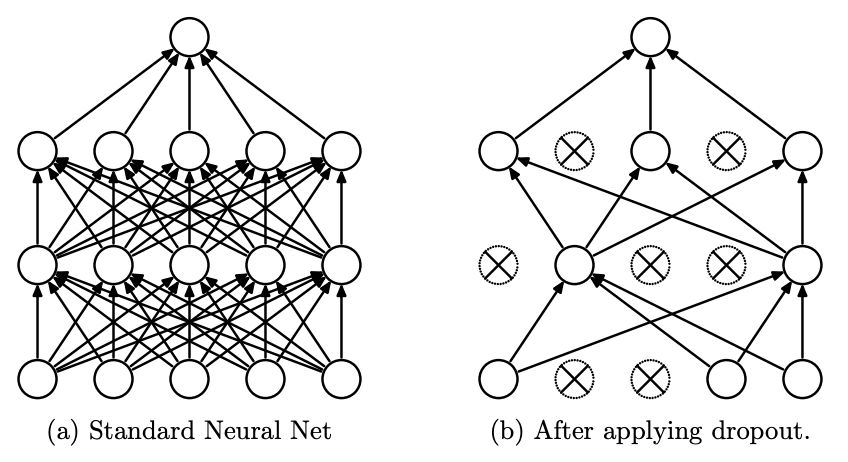
\includegraphics[scale=0.4]{Module 4 (CNN)/pics/dropout.png}

\columnbreak
\begin{itemize}
    \item During training, keep nodes randomly with probability $p$ (usually $p > 0.5$) at each minibatch training. 
    \item During test, use all weights multiplied by $p$.
\end{itemize}
\end{multicols}
\begin{itemize}
    \item Dropout is usually combined with a max-norm regularization that forces the norm of the weights to be under a given maximum value.
\end{itemize}
\end{frame}


\begin{frame}{Data augmentation}
    \begin{itemize}
    \item Generating new training  samples to increase its  diversity. 
    
    \item For images, data augmentation is done by geometric transformations on data: Cropping, flipping, zooming, translations, and blurring specific pixels. 
    
    \item Lighting biases are fixed by color space transformations. 
    \item Deep learning-based data augmentation uses Generative Adversarial Networks (GAN) and feature space augmentations. 
    
    
\end{itemize}
\begin{center}
\begin{tiny}Data augmentation from the CIFAR10 dataset.\end{tiny}

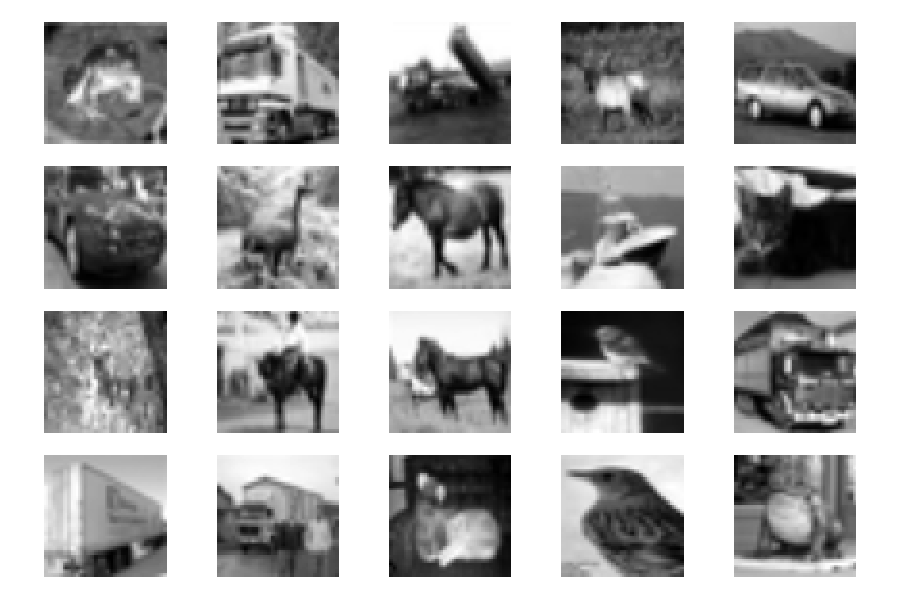
\includegraphics[scale=0.35]{Module 4 (CNN)/pics/data_cifar.pdf}
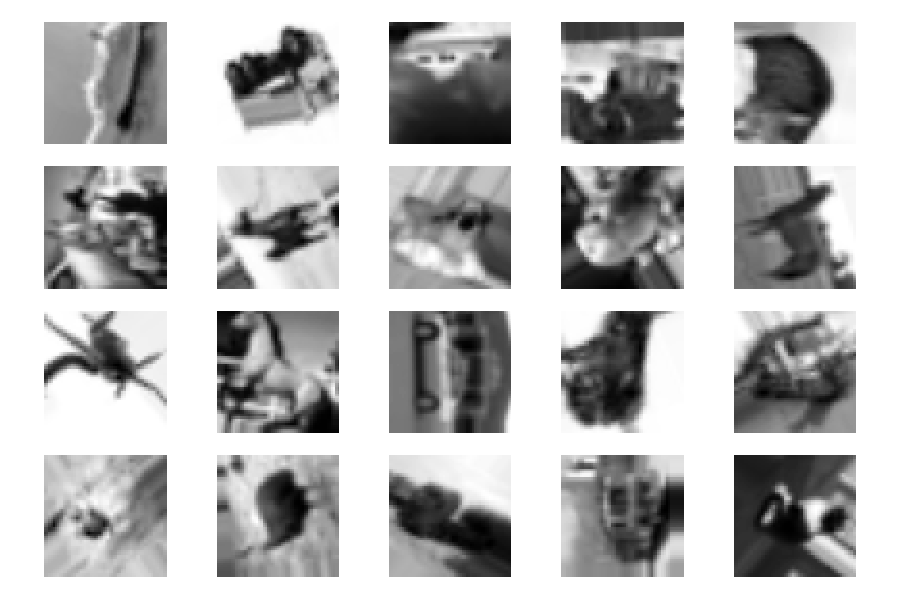
\includegraphics[scale=0.35]{Module 4 (CNN)/pics/data_aug.pdf}\\

\end{center}
\end{frame}

\begin{frame}{Optimizers}{SDG with momentum}
The momentum in an optimizer consists of a fraction of the previous gradient descent. 
\begin{equation}\label{eq:momentum_velocity}
    \bV_{k} = \gamma\bV_{k-1} - \mu \nabla_{\bW} J(\bW_{k}) 
\end{equation}

Parameter $\gamma$ controls the quantity of momentum in the descent. 
\begin{equation}
    \bW_{k+1} = \bW_0 + \sum_{k'=0}^k \bV_{k'} = \bW_{k} + \bV_k
\end{equation}
$\bV$ plays the role of a velocity vector.
\end{frame}

\begin{frame}{Optimizers}{Nesterov Accelerated Gradient}
\begin{itemize}
\item With momentum optimization, if the particle arrives at the minimum, it will keep moving with a vanishing oscillatory movement. 
\item  The Nesterov accelerated gradient descent looks at the gradient one step ahead. The update of the weight vector would be 
\begin{equation}
    \tilde{\bW}_{k+1} = \bW_{k} + \bV_k
\end{equation}
\item The update equations are 
\begin{equation}
\begin{split}
    \bV_k &= \gamma \bV_{k-1} - \mu \nabla_{\bW} J(\tilde{\bW}_k)\\
    \bW_{k+1} & = \bW_k + \bV_k 
\end{split}
\end{equation}
\end{itemize} 
\end{frame}

\begin{frame}{Optimizers}{Adagrad}
\begin{itemize}
\item Adapts the learning rate to each one of the parameters as a function of the norm of the gradient at each one of these parameters. 
\item It first computes the accumulated square value of each component of the gradient 
\begin{equation}
    \bG_k = \bG_{k-1} + \nabla_{\bW}J(\bW_{k}) \odot \nabla_{\bW}J(\bW_{k})
\end{equation}
\item Then, it updates each one of the parameters $w_{i,k}$ in $\bw_k$ as
\begin{equation}
    w_{i,k+1} = w_{i,k} - \frac{\mu}{\sqrt{g_{i,k}}+\varepsilon} \left[\nabla_{\bW}J(\bW_{k})\right]_i
\end{equation}
where $\left[\nabla_{\bW}J(\bW_{k})\right]_i=\frac{d}{dw_{i}}J(\bW_{k})$ is the $i^{th}$ element of the gradient vector and $\varepsilon$ is a small number that is used for numerical stability. 
\end{itemize}
    
\end{frame}

\begin{frame}{Optimizers}{RMSProp}
\begin{itemize}
\item  The AdaGrad algorithm has a learning rate that decreases monotonically with time, which will end up in a learning rate that tends to zero. 

\item The root mean square propagation (RMSProp) algorithm forgets about the squared gradients of remote time instants through an exponential decay
\begin{equation}\label{eq:sq_grad_RMSProp}
    \bG_k = \gamma \bG_{k-1} + \left(1-\gamma\right) \nabla_{\bW}J(\bW_{k}) \odot \nabla_{\bW}J(\bW_{k})
\end{equation}
\item If $\gamma=1$ the algorithm forgets everything about the past gradients. If $\gamma=0$, the algorithm is identic to the AdaGrad one. 
\end{itemize}
\end{frame}

\begin{frame}{Optimizers}{Adam}
    The Adam (Adaptive Momentum Estimation) algorithm is a combination of the previous two ones. 

\begin{equation}
     \bV_{k} = \beta_1\bV_{k-1} - (1-\beta_1) \nabla_{\bW} J(\bW_{k}) 
\end{equation}
\begin{equation}\label{eq:Adam_velocity} 
    \bG_k = \beta_2 \bG_{k-1} + \left(1-\beta_2\right) \nabla_{\bW}J(\bW_{k}) \odot \nabla_{\bW}J(\bW_{k})
\end{equation}
\begin{equation}\label{{eq:sq_grad_Adam}}
    \begin{split}
        \tilde{\bV}_k & = \frac{\bV_k}{1-\beta_1^{k}}\\
        \tilde{\bG}_k & = \frac{\bG_k}{1-\beta_2^{k}}\\
    \end{split}
\end{equation}
 Each element of the weight vector $\bw_k$ is updated as 
\begin{equation}
    w_{i,k+1} = w_{i,k} -\mu \frac{v_{i,k}}{\sqrt{g_{i,k}}+\varepsilon} 
\end{equation}



\end{frame}

\end{document}